% This file was created with tikzplotlib v0.10.1.
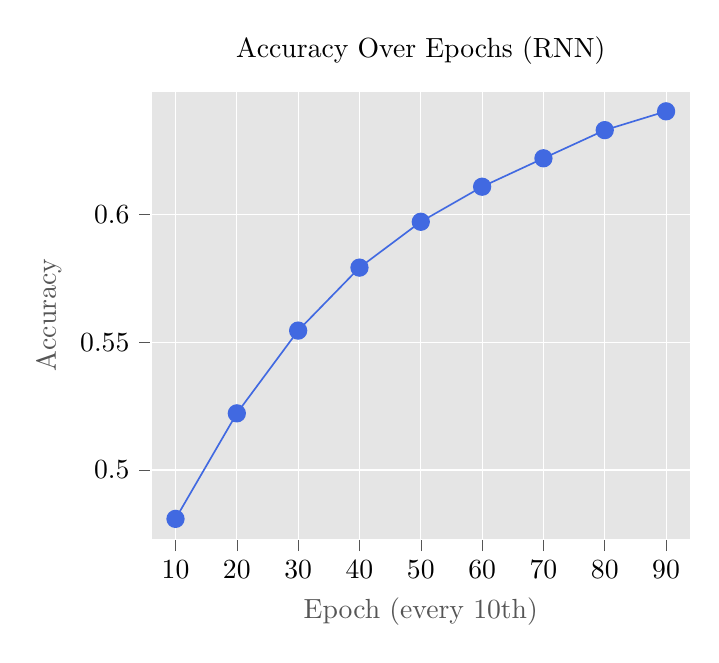
\begin{tikzpicture}

\definecolor{dimgray85}{RGB}{85,85,85}
\definecolor{gainsboro229}{RGB}{229,229,229}
\definecolor{royalblue}{RGB}{65,105,225}

\begin{axis}[
axis background/.style={fill=gainsboro229},
axis line style={white},
tick align=outside,
tick pos=left,
title={Accuracy Over Epochs (RNN)},
x grid style={white},
xlabel=\textcolor{dimgray85}{Epoch (every 10th)},
xmajorgrids,
xmin=-0.4, xmax=8.4,
xtick style={color=dimgray85},
xtick={0,1,2,3,4,5,6,7,8},
xtick={0,1,2,3,4,5,6,7,8},
xticklabels={10,20,30,40,50,60,70,80,90},
xticklabels={10,20,30,40,50,60,70,80,90},
y grid style={white},
ylabel=\textcolor{dimgray85}{Accuracy},
ymajorgrids,
ymin=0.472926071286201, ymax=0.648256549239159,
ytick style={color=dimgray85}
]
\addplot [semithick, royalblue, mark=*, mark size=3, mark options={solid}]
table {%
0 0.480895638465881
1 0.522173941135406
2 0.554530441761017
3 0.57916522026062
4 0.597095668315887
5 0.61080002784729
6 0.621921718120575
7 0.63293045759201
8 0.640286982059479
};
\end{axis}

\end{tikzpicture}
